% This file is generated by the MATLAB m-file laprint.m. It can be included
% into LaTeX documents using the packages graphicx, color and psfrag.
% It is accompanied by a postscript file. A sample LaTeX file is:
%    \documentclass{article}\usepackage{graphicx,color,psfrag}
%    \begin{document}% This file is generated by the MATLAB m-file laprint.m. It can be included
% into LaTeX documents using the packages graphicx, color and psfrag.
% It is accompanied by a postscript file. A sample LaTeX file is:
%    \documentclass{article}\usepackage{graphicx,color,psfrag}
%    \begin{document}% This file is generated by the MATLAB m-file laprint.m. It can be included
% into LaTeX documents using the packages graphicx, color and psfrag.
% It is accompanied by a postscript file. A sample LaTeX file is:
%    \documentclass{article}\usepackage{graphicx,color,psfrag}
%    \begin{document}% This file is generated by the MATLAB m-file laprint.m. It can be included
% into LaTeX documents using the packages graphicx, color and psfrag.
% It is accompanied by a postscript file. A sample LaTeX file is:
%    \documentclass{article}\usepackage{graphicx,color,psfrag}
%    \begin{document}\input{sim1}\end{document}
% See http://www.mathworks.de/matlabcentral/fileexchange/loadFile.do?objectId=4638
% for recent versions of laprint.m.
%
% created by:           LaPrint version 3.16 (13.9.2004)
% created on:           19-May-2007 16:17:51
% eps bounding box:     10.9091 cm x 8.1818 cm
% comment:              
%
\begin{psfrags}%
\psfragscanon%
%
% text strings:
\psfrag{s05}[t][t]{\color[rgb]{0,0,0}\setlength{\tabcolsep}{0pt}\begin{tabular}{c}Time [s]\end{tabular}}%
\psfrag{s06}[b][b]{\color[rgb]{0,0,0}\setlength{\tabcolsep}{0pt}\begin{tabular}{c}Magnetic field [nT]\end{tabular}}%
\psfrag{s10}[][]{\color[rgb]{0,0,0}\setlength{\tabcolsep}{0pt}\begin{tabular}{c} \end{tabular}}%
\psfrag{s11}[][]{\color[rgb]{0,0,0}\setlength{\tabcolsep}{0pt}\begin{tabular}{c} \end{tabular}}%
\psfrag{s12}[l][l]{\color[rgb]{0,0,0}z-directiondirection}%
\psfrag{s13}[l][l]{\color[rgb]{0,0,0}x-directiondirection}%
\psfrag{s14}[l][l]{\color[rgb]{0,0,0}y-directiondirection}%
\psfrag{s15}[l][l]{\color[rgb]{0,0,0}z-directiondirection}%
%
% xticklabels:
\psfrag{x01}[t][t]{-0.3}%
\psfrag{x02}[t][t]{-0.2}%
\psfrag{x03}[t][t]{-0.1}%
\psfrag{x04}[t][t]{0}%
\psfrag{x05}[t][t]{0.1}%
\psfrag{x06}[t][t]{0.2}%
\psfrag{x07}[t][t]{0.3}%
%
% yticklabels:
\psfrag{v01}[r][r]{-150}%
\psfrag{v02}[r][r]{-100}%
\psfrag{v03}[r][r]{-50}%
\psfrag{v04}[r][r]{0}%
\psfrag{v05}[r][r]{50}%
\psfrag{v06}[r][r]{100}%
\psfrag{v07}[r][r]{150}%
%
% Figure:
\resizebox{12cm}{!}{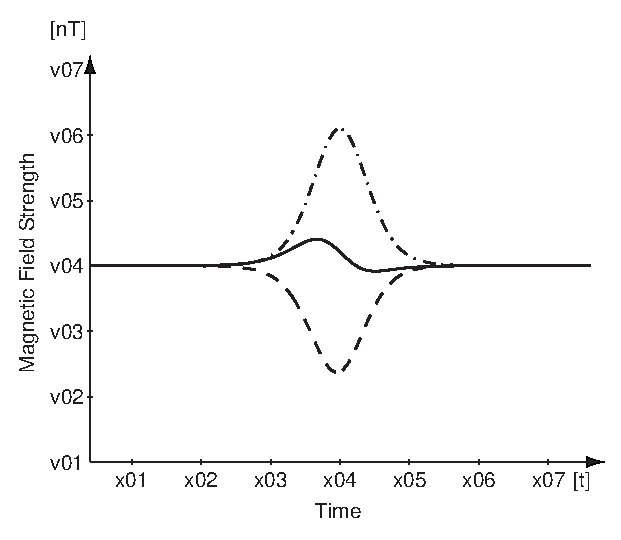
\includegraphics{sim1.eps}}%
\end{psfrags}%
%
% End sim1.tex
\end{document}
% See http://www.mathworks.de/matlabcentral/fileexchange/loadFile.do?objectId=4638
% for recent versions of laprint.m.
%
% created by:           LaPrint version 3.16 (13.9.2004)
% created on:           19-May-2007 16:17:51
% eps bounding box:     10.9091 cm x 8.1818 cm
% comment:              
%
\begin{psfrags}%
\psfragscanon%
%
% text strings:
\psfrag{s05}[t][t]{\color[rgb]{0,0,0}\setlength{\tabcolsep}{0pt}\begin{tabular}{c}Time [s]\end{tabular}}%
\psfrag{s06}[b][b]{\color[rgb]{0,0,0}\setlength{\tabcolsep}{0pt}\begin{tabular}{c}Magnetic field [nT]\end{tabular}}%
\psfrag{s10}[][]{\color[rgb]{0,0,0}\setlength{\tabcolsep}{0pt}\begin{tabular}{c} \end{tabular}}%
\psfrag{s11}[][]{\color[rgb]{0,0,0}\setlength{\tabcolsep}{0pt}\begin{tabular}{c} \end{tabular}}%
\psfrag{s12}[l][l]{\color[rgb]{0,0,0}z-directiondirection}%
\psfrag{s13}[l][l]{\color[rgb]{0,0,0}x-directiondirection}%
\psfrag{s14}[l][l]{\color[rgb]{0,0,0}y-directiondirection}%
\psfrag{s15}[l][l]{\color[rgb]{0,0,0}z-directiondirection}%
%
% xticklabels:
\psfrag{x01}[t][t]{-0.3}%
\psfrag{x02}[t][t]{-0.2}%
\psfrag{x03}[t][t]{-0.1}%
\psfrag{x04}[t][t]{0}%
\psfrag{x05}[t][t]{0.1}%
\psfrag{x06}[t][t]{0.2}%
\psfrag{x07}[t][t]{0.3}%
%
% yticklabels:
\psfrag{v01}[r][r]{-150}%
\psfrag{v02}[r][r]{-100}%
\psfrag{v03}[r][r]{-50}%
\psfrag{v04}[r][r]{0}%
\psfrag{v05}[r][r]{50}%
\psfrag{v06}[r][r]{100}%
\psfrag{v07}[r][r]{150}%
%
% Figure:
\resizebox{12cm}{!}{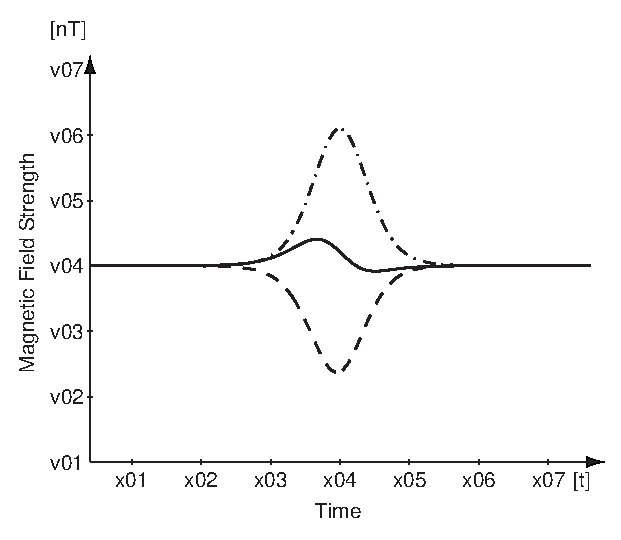
\includegraphics{sim1.eps}}%
\end{psfrags}%
%
% End sim1.tex
\end{document}
% See http://www.mathworks.de/matlabcentral/fileexchange/loadFile.do?objectId=4638
% for recent versions of laprint.m.
%
% created by:           LaPrint version 3.16 (13.9.2004)
% created on:           19-May-2007 16:17:51
% eps bounding box:     10.9091 cm x 8.1818 cm
% comment:              
%
\begin{psfrags}%
\psfragscanon%
%
% text strings:
\psfrag{s05}[t][t]{\color[rgb]{0,0,0}\setlength{\tabcolsep}{0pt}\begin{tabular}{c}Time [s]\end{tabular}}%
\psfrag{s06}[b][b]{\color[rgb]{0,0,0}\setlength{\tabcolsep}{0pt}\begin{tabular}{c}Magnetic field [nT]\end{tabular}}%
\psfrag{s10}[][]{\color[rgb]{0,0,0}\setlength{\tabcolsep}{0pt}\begin{tabular}{c} \end{tabular}}%
\psfrag{s11}[][]{\color[rgb]{0,0,0}\setlength{\tabcolsep}{0pt}\begin{tabular}{c} \end{tabular}}%
\psfrag{s12}[l][l]{\color[rgb]{0,0,0}z-directiondirection}%
\psfrag{s13}[l][l]{\color[rgb]{0,0,0}x-directiondirection}%
\psfrag{s14}[l][l]{\color[rgb]{0,0,0}y-directiondirection}%
\psfrag{s15}[l][l]{\color[rgb]{0,0,0}z-directiondirection}%
%
% xticklabels:
\psfrag{x01}[t][t]{-0.3}%
\psfrag{x02}[t][t]{-0.2}%
\psfrag{x03}[t][t]{-0.1}%
\psfrag{x04}[t][t]{0}%
\psfrag{x05}[t][t]{0.1}%
\psfrag{x06}[t][t]{0.2}%
\psfrag{x07}[t][t]{0.3}%
%
% yticklabels:
\psfrag{v01}[r][r]{-150}%
\psfrag{v02}[r][r]{-100}%
\psfrag{v03}[r][r]{-50}%
\psfrag{v04}[r][r]{0}%
\psfrag{v05}[r][r]{50}%
\psfrag{v06}[r][r]{100}%
\psfrag{v07}[r][r]{150}%
%
% Figure:
\resizebox{12cm}{!}{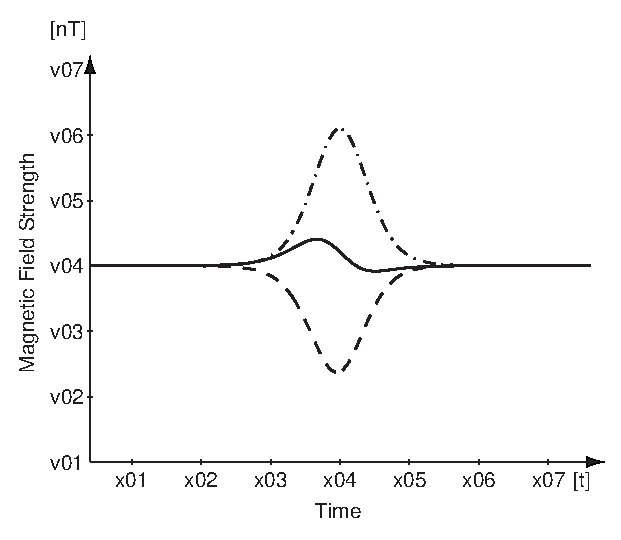
\includegraphics{sim1.eps}}%
\end{psfrags}%
%
% End sim1.tex
\end{document}
% See http://www.mathworks.de/matlabcentral/fileexchange/loadFile.do?objectId=4638
% for recent versions of laprint.m.
%
% created by:           LaPrint version 3.16 (13.9.2004)
% created on:           19-May-2007 16:17:51
% eps bounding box:     10.9091 cm x 8.1818 cm
% comment:              
%
\begin{psfrags}%
\psfragscanon%
%
% text strings:
\psfrag{s05}[t][t]{\color[rgb]{0,0,0}\setlength{\tabcolsep}{0pt}\begin{tabular}{c}Time [s]\end{tabular}}%
\psfrag{s06}[b][b]{\color[rgb]{0,0,0}\setlength{\tabcolsep}{0pt}\begin{tabular}{c}Magnetic field [nT]\end{tabular}}%
\psfrag{s10}[][]{\color[rgb]{0,0,0}\setlength{\tabcolsep}{0pt}\begin{tabular}{c} \end{tabular}}%
\psfrag{s11}[][]{\color[rgb]{0,0,0}\setlength{\tabcolsep}{0pt}\begin{tabular}{c} \end{tabular}}%
\psfrag{s12}[l][l]{\color[rgb]{0,0,0}z-directiondirection}%
\psfrag{s13}[l][l]{\color[rgb]{0,0,0}x-directiondirection}%
\psfrag{s14}[l][l]{\color[rgb]{0,0,0}y-directiondirection}%
\psfrag{s15}[l][l]{\color[rgb]{0,0,0}z-directiondirection}%
%
% xticklabels:
\psfrag{x01}[t][t]{-0.3}%
\psfrag{x02}[t][t]{-0.2}%
\psfrag{x03}[t][t]{-0.1}%
\psfrag{x04}[t][t]{0}%
\psfrag{x05}[t][t]{0.1}%
\psfrag{x06}[t][t]{0.2}%
\psfrag{x07}[t][t]{0.3}%
%
% yticklabels:
\psfrag{v01}[r][r]{-150}%
\psfrag{v02}[r][r]{-100}%
\psfrag{v03}[r][r]{-50}%
\psfrag{v04}[r][r]{0}%
\psfrag{v05}[r][r]{50}%
\psfrag{v06}[r][r]{100}%
\psfrag{v07}[r][r]{150}%
%
% Figure:
\resizebox{12cm}{!}{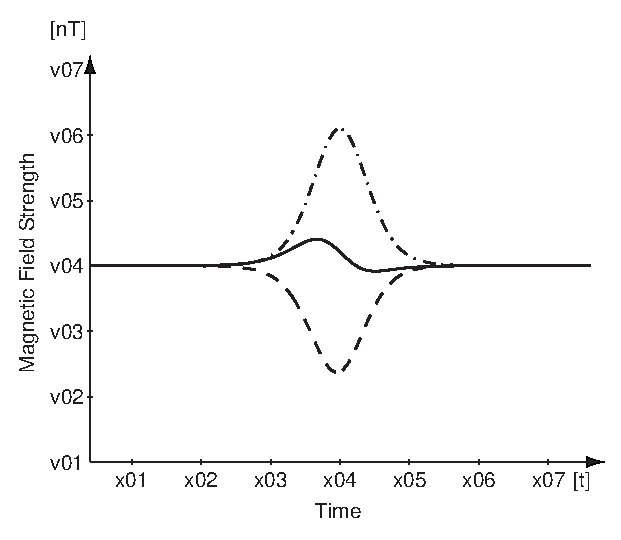
\includegraphics{sim1.eps}}%
\end{psfrags}%
%
% End sim1.tex
